\subsection{Reporting Data Quality Issues}
Data quality issues are identified through a number of mechanisms
including data quality assessment tools, instrument mentors, project
scientists and data users. 
A web-based DQR submission portal was designed to enable easy 
and comprehensive reporting of data quality issues for
any ARM instrument or data stream (Figure~\ref{fig:dqr_tool}). Portal
consists of a complete database of all current and historical
instruments and data streams across ARM facility allowing data quality
report to be submitted for any site, facility, instrument or data stream
at the granularity of specific affected variable and for selected time
period. In addition to the detailed description of the quality issue and
affected variables, portal also allows for corrective update and
maintenance actions to be suggested by the instrument experts.
Suggestion for correcting the data can be provided in form of symbolic
equations. Auto-complete feature of the portal ensures easy and correct
variables names to be used in the symbolic equation, and detect and
capture variable dependencies. Each DQR is assigned an unique identifier
(DQRID) and is recorded within a PostgreSQL database.

\begin{figure}
 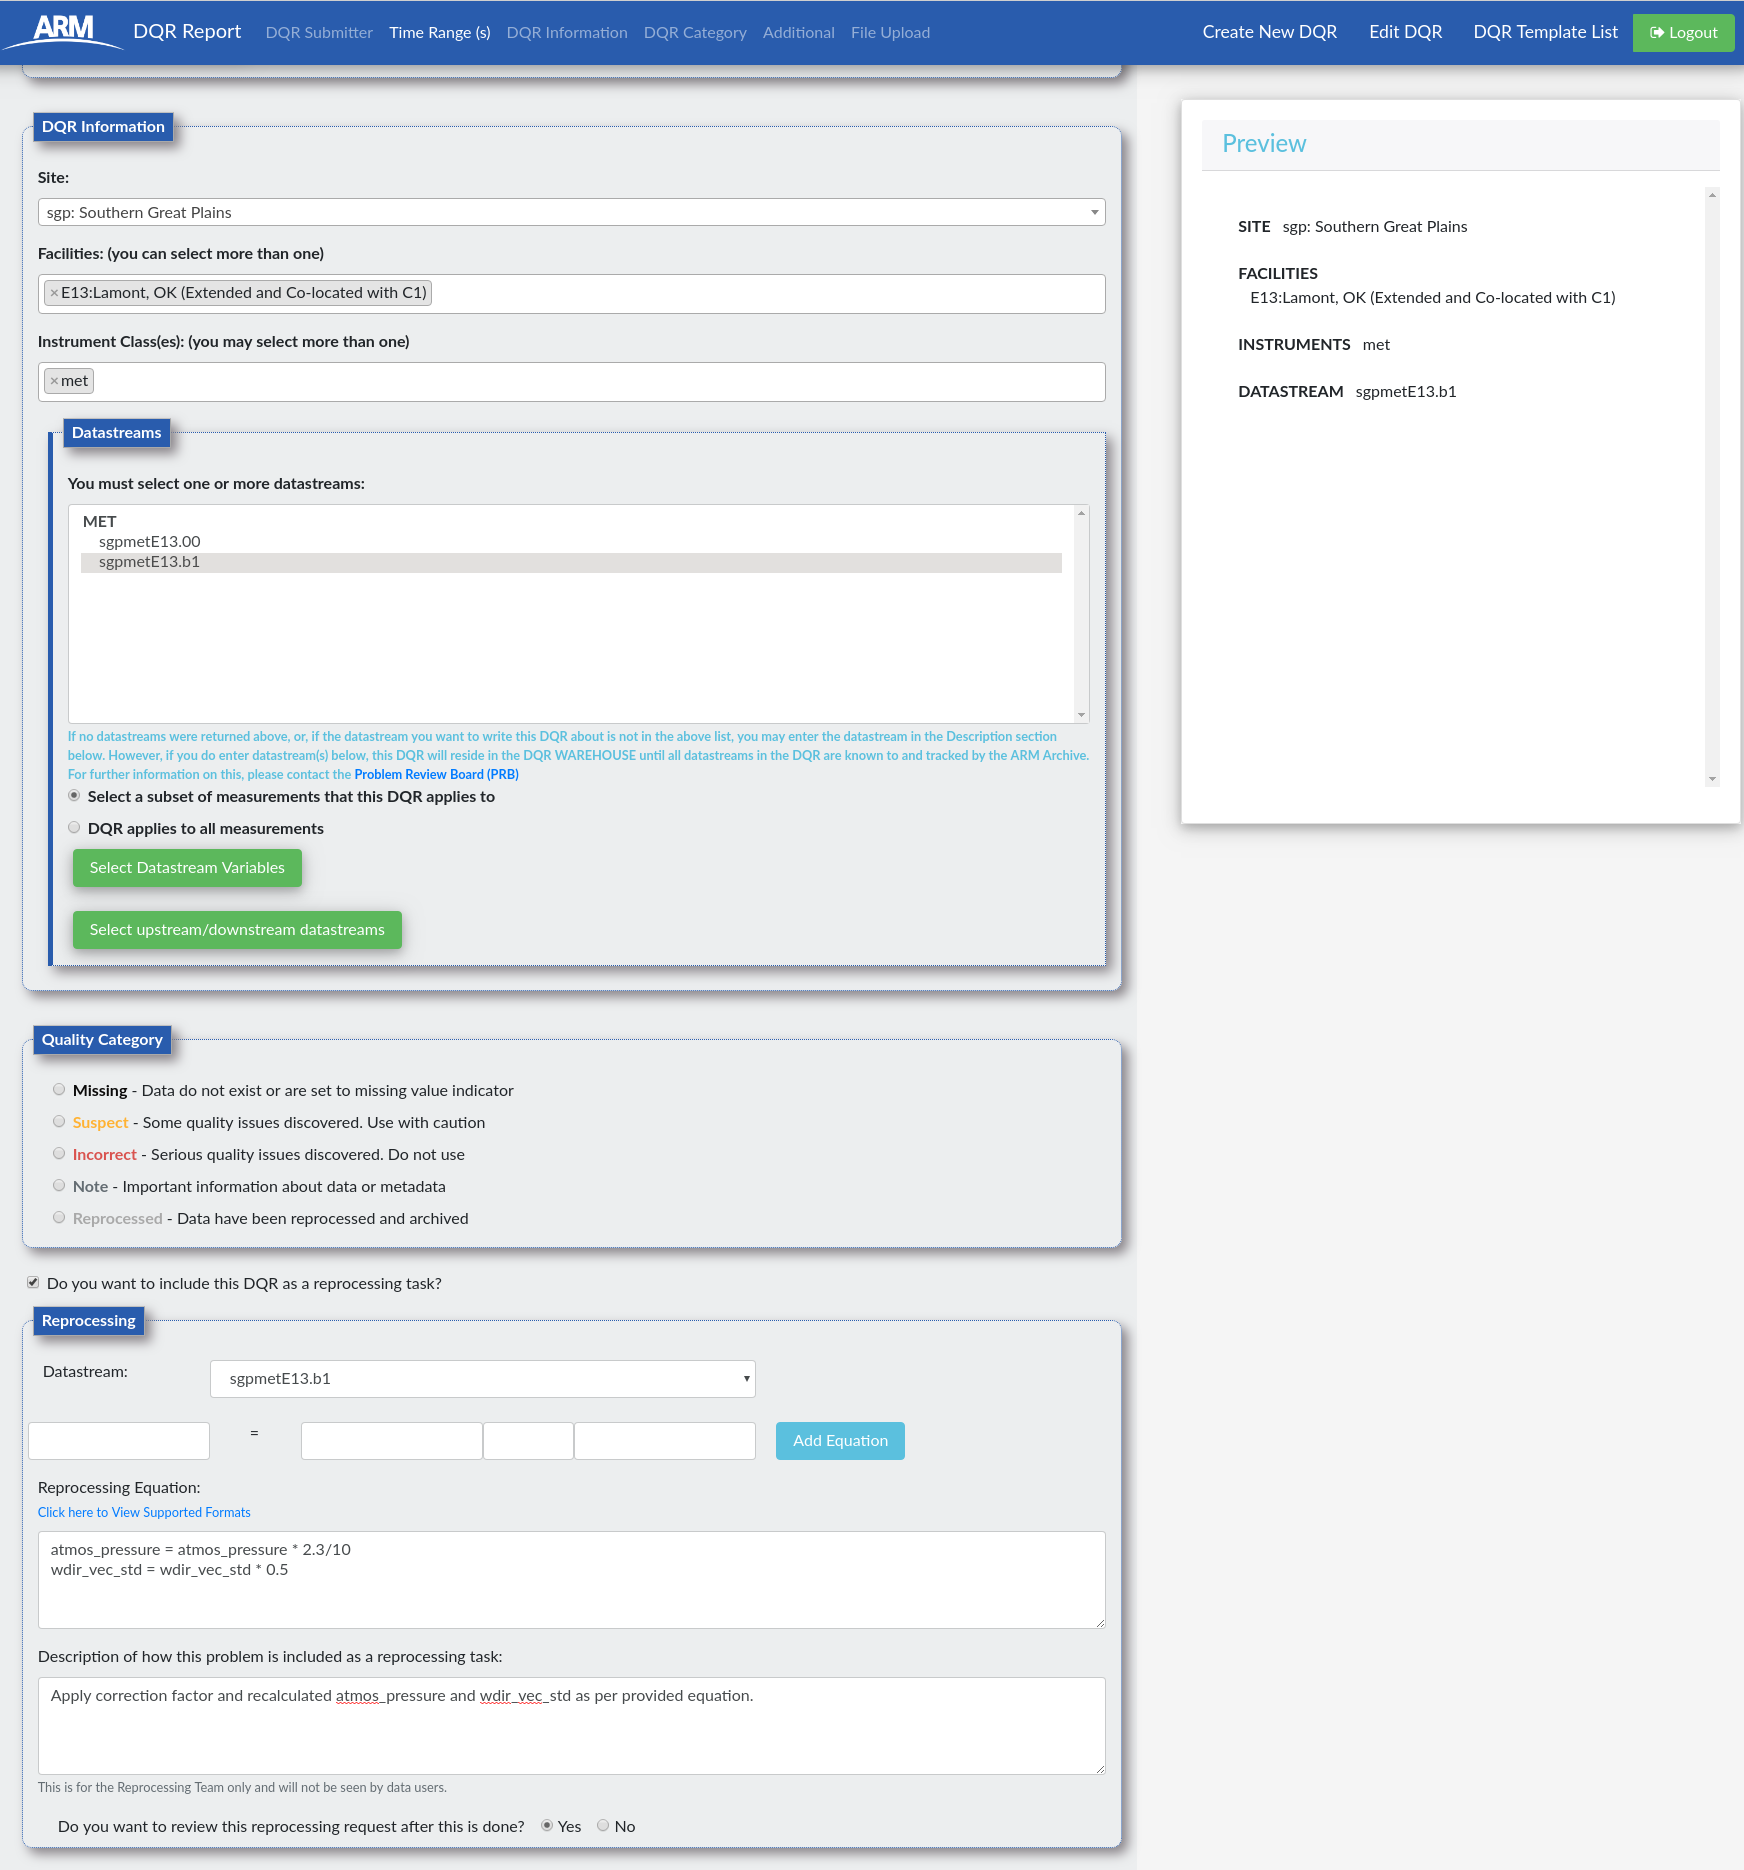
\includegraphics[width=\columnwidth]{figures/dqr_tool.png}
 \caption{DQR Submission Tool allows reporting of data quality issues
	for any observational site, facility and instrument to the
	granularity of individual variable within the data files. Suggestion
 for data correction can be provided in form of symbolic equations which
 be used for automated processing tools to apply the correction.}
 \label{fig:dqr_tool}
\end{figure}
